\documentclass[11pt]{article}
\usepackage[margin=1in]{geometry}
\usepackage{amsmath,amssymb,booktabs,graphicx,float,placeins,subfigure}
\title{Synthetic Legacy Econometric Report}
\author{}
\date{}

\begin{document}
\maketitle

\section{Estimating equations}
The report deliberately retains a legacy preamble and figure syntax while all
substantive content is invented. Let $g$ index groups and $t$ periods. The
estimating system is
\begin{align}
y_{igt} & = \alpha_g + \lambda_t
  + \sum_{k=-3}^{3} \beta_k
    \mathbf{1}\{t-T_g=k\}
  + x_{igt}'\gamma + \varepsilon_{igt}, \label{eq:event} \\
\widehat{\Omega}
  & = (X'X)^{-1}
    \left(\sum_{g=1}^{G} X_g'\widehat{u}_g
    \widehat{u}_g'X_g\right)(X'X)^{-1}. \label{eq:variance}
\end{align}
The normalization is $\beta_{-1}=0$, and the identifying restriction is
$\mathbb{E}[\varepsilon_{igt}\mid X,\alpha_g,\lambda_t]=0$.

\section{Legacy panels}
\begin{figure}[H]
  \centering
  \subfigure[Synthetic outcome]{
    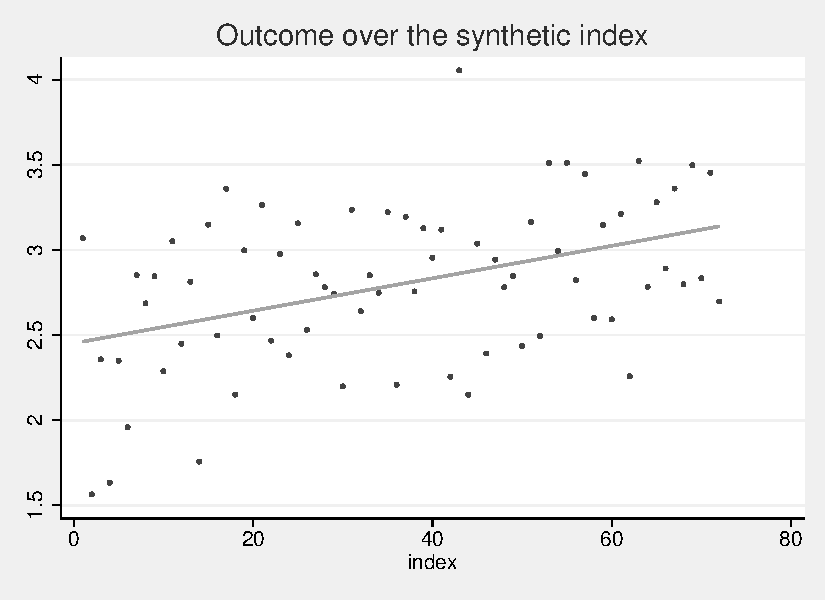
\includegraphics[width=.40\textwidth]{figures/legacy-outcome.pdf}}
  \hfill
  \subfigure[Synthetic exposure]{
    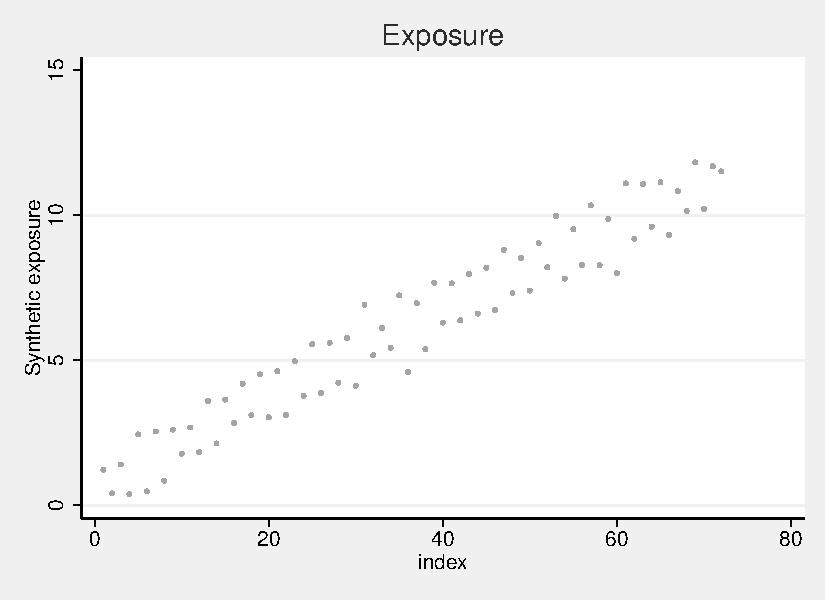
\includegraphics[width=.40\textwidth]{figures/legacy-exposure.pdf}}
  \caption{Legacy subfigure layout}
  \label{fig:legacy}
\end{figure}
\FloatBarrier

\section{Regression output}
\begin{table}[H]
\centering
\caption{Synthetic legacy estimates}
\label{tab:legacy}
\begin{tabular}{lcc}
\toprule
 & Baseline & Controls \\
\midrule
Event coefficient & 0.184 & 0.161 \\
 & (0.052) & (0.049) \\
Exposure coefficient & 0.073 & 0.069 \\
 & (0.021) & (0.020) \\
Observations & 720 & 720 \\
\bottomrule
\end{tabular}

\vspace{2pt}
\begin{minipage}{.82\textwidth}
\footnotesize\textit{Notes:} All values are invented. Parentheses contain
synthetic group-clustered standard errors.
\end{minipage}
\end{table}


Equations~\eqref{eq:event}--\eqref{eq:variance}, Figure~\ref{fig:legacy}, and
Table~\ref{tab:legacy} verify the relative-input and cross-reference paths.

\end{document}
